\section{Praktikos veiklos aprašymas}
Šį skyrių sudaro praktikos veiklos aprašymas ir jos įgyvendinimas.

\subsection{Praktikos vietos gavimas}
Norint gauti praktikos vietą \enquote{Bentley systems} reikėjo atlikti 3 su programavimu susijusias užduotis \enquote{Codility} aplinkoje. Jei šios užduotys buvo atliktos gerai, kandidatas kviečiamas antram etapui. Antrojo etapo metu \enquote{Codility} aplinkoje susipažinama su programuotojais, kurie stebės kandidato užduočių atlikimą, padės jei iškils problemų. Interviu stebintys programuotojai dažniausiai nėra susiję su komanda, kurioje bus atliekama darbo praktika. Prieš pradedant atlikti naujas užduotis, diskutuojamos pirmo etapo užduotys, kas galėjo būti geriau, kodėl tam tikri kodo sprendimai buvo priimti. Po diskusijos pateikiamos pora užduočių, kandidatas bando jas išspręsti, užstrigus, programuotojai padeda. Užduotys olimpiadinio programavimo pobūdžio ir objektinio programavimo pagrindų patikrinimo.

Pirmoji darbo diena prasidėjo nuo terminuotos sutarties pasirašymo. Po to supažindino su komanda, mentoriumi, su kuriuo dirbsiu artimiausius 3 mėnesius. Komandą sudaro 15 narių: 3 testuotojai, 1 projektų vadovas ir 12 įvairaus lygio programuotojų. Kas 3 savaites susitinkama su mentoriumi pasidalinti su per 3 savaites įvykusiais įvykiais, atsiradusiomis problemomis, diskutuojama kaip jos galėtų būti išspręstos.

% Praktikos veiklos aprašymas (vienas arba keli skyriai). Aprašomas praktikos užduoties įgyvendinimas (pvz., atlikti projektavimo ir/ar programavimo darbai, sukurtas modelis, priimti sprendimai ir pan.).

\newpage

\subsection{Praktikos metu naudotos technologijos}
Šiame poskyryje aprašomos technologijos, kurias naudojau praktikos metu ir pavyzdžiai, kur jos buvo naudojamos. 
Atlikdamas praktiką mobiliųjų įrenginių kūrimo komandoje turėjau galimybę dirbti su įvairiomis pripažintomis ir naujausiomis technologijomis. Toliau aprašoma pagrindinių \enquote{Android} ir \enquote{iOS} technologijų, kuriomis naudojausi, apžvalga:

Jetpack Compose yra modernus Google vartotojo sąsajų priemonių rinkinys, skirtas Android taikomųjų programų vartotojo sąsajoms kurti. Jame naudojamas deklaratyvusis metodas, kai kūrėjai aprašo norimą naudotojo sąsajos būseną, o ne tai, kaip ją pasiekti žingsnis po žingsnio. Taikant šį požiūrį kodas gali būti glaustesnis ir lengviau suprantamas.  "Jetpack Compose" naudoja "Kotlin" galimybes, todėl kūrėjai gali kurti vartotojo sąsajos komponentus kaip funkcijas.  Tai gali pagerinti kodo skaitomumą ir palaikymą.


\subsubsection{Kotlin}
Kotlin yra viena iš populiariausių programavimo kalbų kuriant Android mobiliąsias programėles. Lyginant su Java programavimo kalba, Kotlin yra modernesnė, null reikšmių saugumu. Kotlin lengvai pritaikoma senesniuose projektuose, parašytuose su Java ir XML vartotojo sąsaja, paprasta atnaujinti seną kodo bazę. Sintaksės panašumas į kitas programavimo kalbas, padeda lengvai ir greita išmokti Kotlin programavimo kalbos pagrindus.
Visos praktikos metu Kotlin programavimo kalbą naudojau kurti naudotojo sąsajos logiką, tvarkyti duomenis ir integruoti naujus komponentus į turimą mobiliąją programėlę.

\subsubsection{Jetpack Compose}

"Jetpack Compose" yra Android rekomenduojamas modernus įrankių rinkinys, skirtas vietinei vartotojo sąsajai kurti. Rinkinys supaprastina ir pagreitina Android mobiliųjų programėlių vartotojo sąsajos kūrimą. Jame taikomas deklaratyvus metodas,

% % \begin{figure}
% %     \centering
% %     \begin{minted}[linenos,tabsize=1,breaklines]{kotlin}
% %     @Composable
% %     fun TestListParameterView(
% %         values: List<String>,
% %         initialMessage: String = "Initial message",
% %         labelText: String = "Label",
% %         onRemove: (String) -> Unit,
% %         onAdd: (String) -> Unit
% %     ) {
% %         var text by rememberSaveable { mutableStateOf(initialMessage) }
% %         Column {
% %             LazyColumn(modifier = Modifier.height(200.dp)) {
% %                 items(items = values) { value ->
% %                     Row {
% %                         Text(
% %                             modifier = Modifier.height(44.dp).fillMaxWidth(0.9f),
% %                             maxLines = 2,
% %                             style = MaterialTheme.typography.body2,
% %                             text = value,
% %                             overflow = TextOverflow.Ellipsis
% %                         )
% %                         Spacer(modifier = Modifier.weight(1f))
% %                         TextButton(
% %                             modifier = Modifier.width(44.dp).background(Color.Transparent),
% %                             onClick = { onRemove(value) },
% %                             content = { Icon(painter = painterResource(...)) }
% %                         )
% %                     }
% %                 }
% %             }
% %             OutlinedTextField(
% %                 modifier = Modifier.fillMaxWidth(),
% %                 value = text,
% %                 onValueChange = { text = it },
% %                 label = { Text(labelText) }
% %             )
% %             Button(onClick = {
% %                 if (text.isNotBlank()) {
% %                     onAdd(text)
% %                     text = ""
% %                 }
% %             }) { Text(text = "Add") }
% %         }
% %     }
% %     \end{minted}
% %     \caption{Jetpack Compose programinis kodas}
% %     \label{fig:composeCode}
% % \end{figure}

% % \begin{figure}[htbp!]
% %   \centering
% %   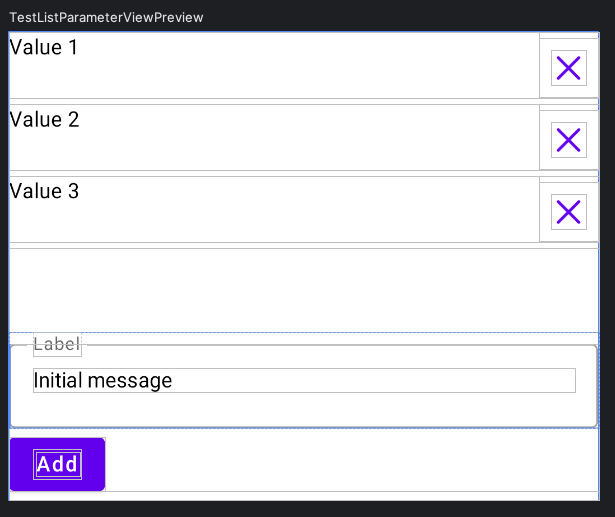
\includegraphics[width=0.8\linewidth]{Images/JetpackCompose.png}
% %   \caption{Jetpack Compose komponento peržiūra}
% %   \label{fig:example}
% % \end{figure}


\subsubsection{Swift}
Swift yra galinga, tačiau nesunki pradedantiesiems programavimo kalba, kurią Apple sukūrė savo įrenginiams. Lyginant su \enquote{Objective-C}, Swift pasižymi švariu ir glaustu stiliumi, artimesniu natūraliai kalbai. Priešingai nei \enquote{Objective-C}, Swift atlieka daugiau automatinio atminties valdymo ir tipų tikrinimo, tai padeda išvengti gedimų ir klaidų, kurios dažniau pasitaiko \enquote{Objective-C} kalboje. Dėl šių priežasčių, dėmesio, programinį kodą  greita parašyti ir lengva prižiūrėti. Nors \enquote{Objective-C} dar naudojama esamuose projektuose, integruoti Swift nesunku net ir į itin senus projektus. Su Swift programavimo kalba galima rašyti programėles iPhone, iPad, MacBook, Apple watch įrenginiams. Neseniai atsiradusiam \enquote{Apple vision pro} prietaisui irgi yra galimybė kurti programas šia programavimo kalba. 

\subsubsection{SwiftUI}

\enquote{SwiftUI} - tai naujas Apple karkasas įrenginių naudotojo sąsajų kūrimui. Skirtingai nuo storyboards sąsajų kūrimo, kuris remiasi vizualiniu komponentų dėliojimu ekrane, \enquote{SwiftUI} naudoja deklaratyvų požiūrį. Storyboards vartotojo sąsajos konvertuojamos į XML,  kas yra gana nepatogu, kai atliekamos programinio kodo pakeitimų peržiūros. Kaip ir \enquote{Jetpack compose}, \enquote{SwiftUI}, kode galima atlikti vartotojo sąsajos būsenų valdymą, deklaratyviai konstruoti vartotojo sąsają. Išbandžius abi technologijas iOS vartotojo sąsajos kūrimo technologijas, norint suprasti ir atlikti kodo pakeitimus esamame projekte, \enquote{SwiftUI} yra geresnis programavimo karkasas, suprasti kodo veikimo principus, prireiks mažiau laiko.

\subsection{Praktikos užduotys}

Šiame poskyryje pateiktos visos užduotys, kurios buvo atliktos praktikos metu. Kiekviena užduotis bus trumpai apibūdinta, įvardinant jos tikslą, įgyvendinimo būdus ir pasiektus rezultatus mobiliojoje programėlėje. Programinis kodas, kuris yra pateiktas sekančiuose skyreliuose yra tik iškarpos, siekiant parodyti pagrindinį funkcionalumą.
\subsubsection{Programinio kodo klaidos (\emph{angl. bugs})}
\subsubsubsection{Programinio kodo klaidų radimas}
Synchro Field projektas yra padalintas į 2 dalis: Android ir iOS. Praktikos metu, atliekant užduotis abiejose platformose, mobiliosios programėlės funkcionalumai turi būti kuo labiau suvienodinti. Testuojant savo atliktų užduočių pakeitimus, teko pastebėti tam tikrus neatitikimus vienoje iš platformų. Tiesa, įgūdis pastebėti kažkokius netikėtus pokyčius mobiliosiose programėlėse įgyjamas ilgiau dirbus su programėlės projektu, nes ne visus funkcionalumus galima iš karto pamatyti. Dažnai randamos klaidos išjungus interneto prieigą, pasukus prietaisą, ar išeinant iš programėlės ir grįžtant į ją atgal.


Radus programinio kodo klaidas, \enquote{AzureDevOps} platformoje sukuriama užduotis, pažingsniui aprašoma, kaip galima atkurti klaidą prietaisuose, ką paspausti, kokio rezultato norima ir koks yra matomas. Parašoma kokioje projekto versijoje rasta klaida, ant kokių mobiliųjų įrenginių pastebėta klaida. Kasdieninio komandos susitikimo metu naujos klaidos yra aptariamos, nustatomos jų sunkumas, ar svarbu atlikti pakeitimus ir sutvarkyti klaidą, kiek galima greičiau. Po diskusijos užduotis priskiriama tam tikrai užduoties atlikimo sričiai.

\subsubsubsection{Programinio kodo klaidų taisymas}
Pasiėmus programinio kodo klaidos užduotį, pirmiausia identifikuojama sritis kur klaida įvyksta. Bandoma išsiaiškinti ar klaida įvyksta dėl specifinės mobiliojo prietaiso versijos ar įvyksta bet kokiu atveju. Jei klaidos nepavyksta pakartoti, kontaktuojama su testuotojais, kad klaida būtų atidžiau patikrinta. 

Praktikos metu, daugiausia klaidų buvo sutvarkyta Pdf dokumento lange. Pateikiamas keletas klaidų kurios buvo sutvarkytos:
\begin{enumerate}
    \item Specifinės anotacijos, pasirinkus anotacijų sąraše pritraukia pdf dokumentą.
    \item Suvienodinta ilgų tekstų trumpinimas į pabaigos pakeitimą į \enquote{...}.
    \item Pasukus Pdf dokumentą trumpam matoma baltas stačiakampis ekrane.
\end{enumerate}

\subsubsection{Užduotis: \enquote{Tap to fullscreen on iOS}}

Ši užduotis buvo skirta realizuoti programos lango pakeitimą į pilno ekrano režimą spustelėjus ant tuščios dokumente vietos, Pdf peržiūros lange. Užduotis buvo paskirstyta į 2 dalis: Android ir iOS. Pasirinkau realizuoti funkcionalumą iOS prietaisuose.

Reikalavimai atliekant užduotį:

\begin{enumerate}
    \item PdfTron anotacijų sąrašas:
    \begin{enumerate}
        \item Komponentų paslėpimas: \enquote{PdfTron}, \enquote{Synchro field} navigacijos, statuso juosta ir apatinė anotacijų juosta turėtų būti paslėpti, kai pdf ekranas apima visą ekraną.
        \item Pdf užimti visą ekraną ir sugrįžti atgal į normalią būseną.
    \end{enumerate}
    \item Kai anotacijų sąrašas atidarytas (telefone):
    \begin{enumerate}
        \item Turėtų elgtis taip pat, tik anotacijų sąrašas turi irgi dingti, kai Pdf ekranas užima visą ekraną.
    \end{enumerate}
    \item Kai anotacijų sąrašas atidarytas (plančetiniame):
    \begin{enumerate}
        \item Turėtų elgtis taip pat, tik šoninio anotacijų sąrašo neuždaryti.
    \end{enumerate}
\end{enumerate}


\enquote{Synchro Field} projekte norint peržiūrėti Pdf failus naudojame biblioteką \enquote{PdfTron} (\ref{fig:pdfViewController screen} priedo paveikslėlis). Tačiau, \enquote{PdfTron} komponento navigacijos juosta yra atskirta nuo \enquote{Synchro field} navigacijos juostos (\ref{img:pdfViewController} priedo paveikslėlis). Reikėjo pridėti pakeitimus funkcijai, kuri įvykdoma, kai \enquote{PdfTron} navigacijos juostos matomumas pasikeičia. \ref{fig:pdfTronCode} paveikslėlyje galime matyti, kad funkcijai pradėjus vykdymą, naudojama \textit{UIView.animate()} funkcija, kuri sklandžiai suanimuoja vartotojo sąsajos pasikeitimus. Patikrinama ar naujas funkcionalumas yra įjungtas su \enquote{feature flag}. Atliekami \enquote{Synchro field} navigacijos juostos apribojimų reikšmių pakeitimai. Animacijos trukmė parinkta 0,2 sekundės, siekiant sulyginti \enquote{PdfTron} ir \enquote{Synchro field} navigacijos laukų animacijų trukmes. Jei anotacijų sąrašas yra atidarytas (\ref{img:annotationList} priedo paveikslėlis), sąrašas paslepiamas.

Šio funkcionalumo programavimo metu teko ne tik rašyti kodą, bet ir išmokti naudotis \enquote{Storyboards}. \enquote{PdfTron} lange reikėjo pridėti papildomų apribojimų (\emph{angl. constraints}), siekiant padidinti Pdf komponento dydį.


\begin{figure}[htbp!]
    \centering
\begin{minted}[linenos,tabsize=1,breaklines]{swift}
extension PdfTronViewController: PdfTronNavigationControllerDelegate {
    // In this function we implement the PDFTronNavigationControllerDelegate protocol to handle the navigation bar visibility
    func pdfTronNavigationController(didSetNavigationBarHidden isHidden: Bool) { 
        UIView.animate(withDuration: 0.2) { [weak self] in // We use 0,2 seconds since it's the same duration as the PDF panel animation duration
            guard let self else { return }
            if Features.isEnabled(DevelopmentFeatureFlag.pdfMarkupNative) { // We only need to handle the navigation bar visibility if the PDFMarkupNative feature is enabled
                labeledBottomBarHeightConstraint.isActive = isHidden
            }
            setNavigationBarVisibility(isHidden)
            view.layoutIfNeeded()
        }

        // If the panel is not closed we need to toggle the panel visibility on tap, in other case the panel will be hidden regardless of the navigation bar visibility
        if let resizablePanelViewController, resizablePanelViewController.panelStatus != .closed { 
            let panelHeight = isHidden ? 0 : resizablePanelViewController.heightHalfExpanded
            resizablePanelViewController.animatePanelToHeight(panelHeight)
        }
    }

    private func setNavigationBarVisibility(_ isHidden: Bool) {
        // In this function we handle the navigation bar and status bar visibility using constraints and expand pdf view to fill the screen
        setStatusBarHidden(isHidden)
        if Features.isEnabled(DevelopmentFeatureFlag.pdfMarkupNative) {
            navigationBarTopConstraint.isActive = isHidden
            navigationBarSafeAreaTopConstraint.isActive = !isHidden
            navigationBarShowingConstraint.constant = isHidden ? 0 : navigationBarHeight
        }
    }
}
\end{minted}
\caption{PdfTronViewController matomumo kodas}
    \label{fig:pdfTronCode}
\end{figure}

\newpage
    
\subsubsection{Užduotis: \enquote{UIButton configuration}}
Ši užduotis buvo skirta perkelti didžiąją dalį mygtukų iOS projekte į FieldUIComponents projektą ir suvienodinti stilių nustatymą naudojant \enquote{UIButton.Configuration}.

Reikalavimai atliekant užduotį:
\begin{enumerate}
    \item Perkelti mygtuko vartotojo sąsajos kodą į FieldUIComponents projektą.
    \item Atnaujinti Field projekto kodo bazę su naujais mygtukų komponentais.
    \item Vizualių pakeitimų neturi būti.
\end{enumerate}

Pirmiausia buvo pereita per visą projektą, pažymėtos vietos, klasių mygtukai, kurie galėtų būti perkelti į FieldUIComponents projektą. Perkėlus mygtukus, buvo perrašyti jų stiliaus nustatymai su \enquote{UIButton.Configuration} (\ref{fig:Primary button} paveikslėlis). Teksto spalvos, šrifto ir dydžio nustatymas negalėjo būti perrašytas \enquote{UIButton.Configuration} pagalba, nes pakeitus mygtuko tekstą, reikšmės įgavo pradines stiliaus reikšmes. 

\begin{figure}[htbp!]
    \centering
    \begin{minted}[linenos,tabsize=1,breaklines]{swift}
@IBDesignable public class PrimaryButton: BaseUIButton {
    override func sharedInit() {
        // First we create UIButton.Configuration instance with plain style, then apply needed style properties
        var configuration = UIButton.Configuration.plain()
        configuration.background.cornerRadius = 3
        configuration.background.backgroundColor = UIColor(fieldColor: .blueCerulean)
        configuration.titleLineBreakMode = .byTruncatingMiddle
        self.configuration = configuration
        // Since the title font, color using the UIButton.Configuration resets on text change, we need set it differently
        setAttributedTitle(font: UIFont.openSans(ofSize: 14), foregroundColor: UIColor(fieldColor: .white))
    }
    ...
}
    \end{minted}
    \caption{Primary button kodo perrašymas naudojant UIButton.Configuration}
    \label{fig:Primary button}
\end{figure}


Taip pat buvo sukurtas FieldUIComponentsApp langas, kuriame galima rasti visus projekte naudojamus mygtukus (\ref{fig:buttonsView.png} priedo paveikslėlis). Kadangi mygtukų langas parašytas su SwiftUI, o patys mygtukai su UIKit funckijomis, reikėjo sukurti \textit{ButtonViewRepresentable}, kuris pasirinktą UIView komponento klasė supakuojama į SwiftUI komponentą, realizavus \textit{UIViewRepresentable} klasės funkcijas (\ref{fig:buttonViewRepresentable} paveikslėlis).

Paveikslėlyje galima matyti kairėje esantį UIKit parašyto komponento SwiftUI apvalkalą (\emph{angl. wrapper}), kurio dėka, dešinėje nuotraukos pusėje galima iškart matyti net UIKit komponento pakeitimus, nepaleidus mobiliosios programėlės. Tai leidžia pagreitinti užduoties atlikimą, nes projekto kompiliavimas ir mobiliosios programėlės diegimas užtrunka daug laiko, didėjant projekto mąstui.

\begin{figure} [htbp!]
    \centering
    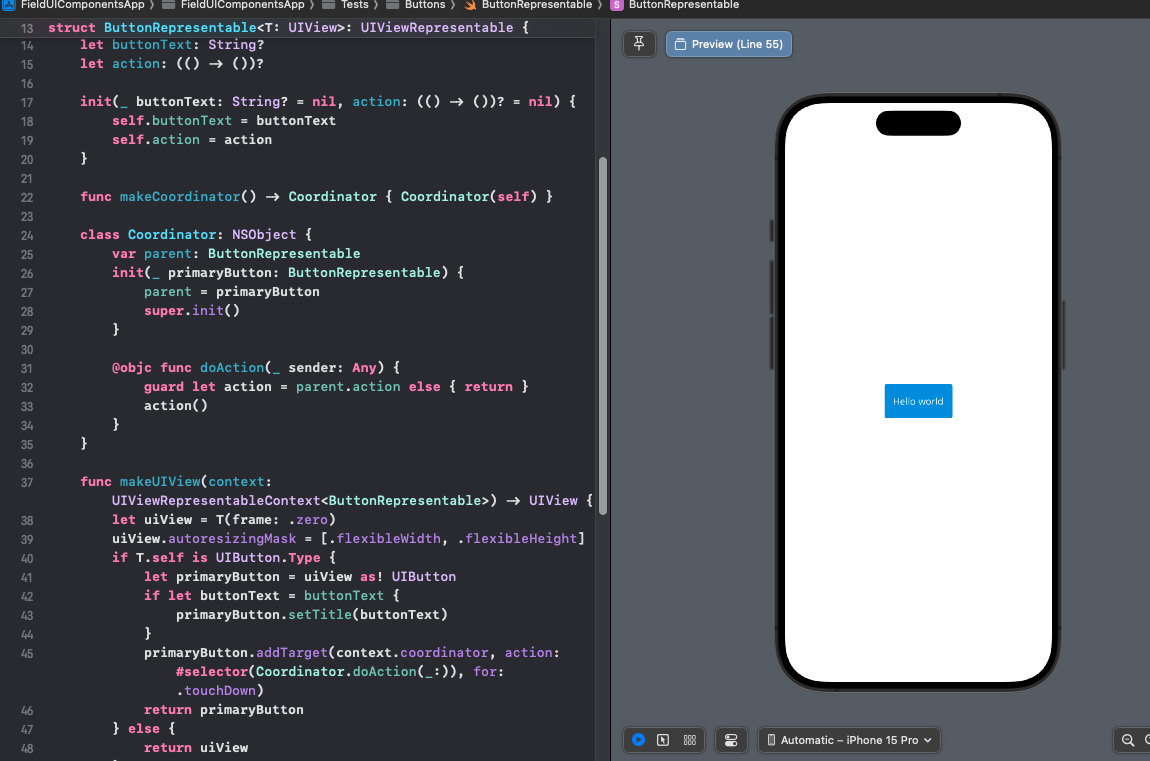
\includegraphics[width=1\textwidth]{Images/iOSButtonRepresentable.png}
    \caption{Vieno mygtuko, parašyto UIKit karkasu atvaizdavimas SwiftUI komponente}
    \label{fig:buttonViewRepresentable}
\end{figure}

\newpage
\subsubsection{Užduotis: \enquote{Custom Toast message on Android}}
Ši užduotis buvo skirta realizuoti UX sukurtą iššokančių žinučių (\emph{angl. Toast messages}) komponentą Android ir iOS operacinėse sistemose. 
Buvo sukurti FieldUIComponents app langai, kuriuose galima įvairiais būdais ištestuoti iššokančias žinutes.

Pasirinkau atlikti šią užduotį Android prietaisuose. 

Reikalavimai atliekant užduotį:
\begin{enumerate}
    \item Sukurti padengtą testais FieldUIComponents komponentą.
    \item Sukurti naują iššokančių žinučių komponentą.
    \begin{enumerate}
        \item Teksto žinutė
        \begin{enumerate}
            \item Tekstas turi tilpti į vieną eilutę.
            \item Jei tekstas užima daugiau vietos, sutrumpinti su \enquote{...}.
            \item Komponento animacija turi kiek galima daugiau sutapti su maketo animacijomis.
        \end{enumerate}
        \item Iššokančios žinutės animacijos trukmė - 3 sekundės.
        \item Iššokančią žinutę galima paslėpti paspaudus ant jos ar atlikus tempimo į viršų gestą.
    \end{enumerate}
    \item Iššokančių žinučių eilė:
    \begin{enumerate}
        \item Iššokančios žinutės patenka į eilę, rodomos viena po kitos, paslepiamos tokia pačia tvarka kaip ir buvo parodytos.
        \item Tokios pačios žinutės nerodomos 2 kartus.
    \end{enumerate}
\end{enumerate}
\newpage
Iš pradžių buvo sukurtas iššokančios žinutės komponentas (\ref{fig:pill} priedo paveikslėlis). Komponentui pritaikytos gestų atpažinimo, paspaudimo funkcionalumas, teksto sutrumpinimas (\ref{fig:pillCode} paveikslėlis).

\begin{figure}[htbp!]
    \centering
    \begin{minted}[linenos,tabsize=1,breaklines]{kotlin}
@Composable
fun Pill(
    modifier: Modifier = Modifier,
    text: String,
    fontSize: TextUnit = dimensionResource(id = R.dimen.toast_font_size).value.sp,
    horizontalPadding: Dp = dimensionResource(id = R.dimen.toast_padding_horizontal),
    verticalPadding: Dp = dimensionResource(id = R.dimen.toast_padding_vertical)
) {
    // We create a surface to clip the content of the pill, with UX defined padding, circular shape and background color
    Surface(
        modifier = modifier
            .padding(horizontal = horizontalPadding),
        shape = CircleShape,
        color = colorResource(R.color.toastBackground)
    ) {
        Row(
            modifier = Modifier
                .wrapContentWidth()
                .padding(horizontalPadding, verticalPadding),
            horizontalArrangement = Arrangement.Center
        ) {
            // Text composable is set to display truncated text if it exceeds the width of the pill, with a max of 1 line
            Text(
                text = text,
                textAlign = TextAlign.Center,
                fontSize = fontSize,
                color = Color.White,
                style = MaterialTheme.typography.body2,
                maxLines = 1,
                overflow = TextOverflow.Ellipsis
            )
        }
    }
}
    \end{minted}
    \caption{Iššokančios žinutės komponento kodas}
    \label{fig:pillCode}
\end{figure}
\newpage
Sukurtas \enquote{ToastViewModel}, kuris rūpinasi iššokančių žinučių eile, patikrina eilėje esančias žinutes, jei eilėje egzistuoja žinutė, antrą kartą jos neparodys (\ref{fig:ToastViewModel} paveikslėlis). Taip pat galima pateikti žinutės trukmę. Pasibaigus trukmei, žinutė išmetama iš eilės.

\begin{figure}[htbp!]
    \centering
    \begin{minted}[linenos,tabsize=1,breaklines]{kotlin}
class ToastViewModel : ViewModel() {
    private val _toastDataState = MutableStateFlow<ToastData?>(null)
    val toastDataState = _toastDataState.asStateFlow()

    private val mutex = Mutex()

    private var pendingMessages: MutableSet<String> = mutableSetOf()

    // This function handles the toast queue with defined duration and message
    fun showToast(
        message: String,
        duration: Long = 3000L
    ) {
        // if the message is already in the queue, don't add it again
        if (pendingMessages.isEmpty() || pendingMessages.last() != message) {
            pendingMessages.add(message)
            viewModelScope.launchSafe {
                mutex.withLock {
                    try {
                        // Create cancellable coroutine to wait for the toast to be dismissed
                        return@launchSafe suspendCancellableCoroutine { continuation ->
                            _toastDataState.value = ToastData(message, duration, continuation)
                        }
                    } finally {
                        // When toast is dismissed, remove it from the queue
                        _toastDataState.value = null
                        pendingMessages.remove(message)
                    }
                }
            }
        }
    }
}
    \end{minted}
    \caption{ToastViewModel programinis kodas}
    \label{fig:ToastViewModel}
\end{figure}

\newpage
Buvo sukurtas \enquote{ToastHost}, skirtas tvarkingai, su animacijomis parodyti iššokančias žinutes  (\ref{fig:ToastHost} paveikslėlis). Panaudota 1,5 konstanta, kad paslėptų iššokančią žinutę, kai kyla į viršų už navigacijos juostos. Standumo ir kiti animacijos parametrai parinkti, kad kuo labiau atitiktų Figma maketų animacijas.

\begin{figure}[htbp!]
    \centering
    \begin{minted}[linenos,tabsize=1,breaklines]{kotlin}
...
// We define the spring animation for enter and exit animations, 1.5 constant is used to hide the toast behind the screen when dismissed
val animationOffset: (Int) -> Int = { (heightToDropPx + it * 1.5).toInt() * -1 }
val springAnimationSpec: FiniteAnimationSpec<IntOffset> = spring(
    dampingRatio = Spring.DampingRatioMediumBouncy,
    stiffness = Spring.StiffnessMedium
)

// Launch effect to show and hide the toast with the given duration
LaunchedEffect(currentToastData) {
    setVisibility(true)
    delay(currentToastData.duration)
    setVisibility(false)
}

// Handle animated visibility of the toast using springAnimationSpec animation
AnimatedVisibility(
    modifier = modifier.padding(top = heightToDrop),
    enter = slideInVertically(springAnimationSpec, initialOffsetY = animationOffset),
    exit = slideOutVertically(springAnimationSpec, targetOffsetY = animationOffset),
    visibleState = isVisible,
    content = { toast() }
)
...
    \end{minted}
    \caption{ToastHost programinis kodas}
    \label{fig:ToastHost}
\end{figure}

\newpage
Kadangi \enquote{Jetpack Compose} komponentų nepavyksta tiesiogiai integruoti į fragmentais pagrįstą programėlę, reikėjo sukurti papildomą klasę \enquote{Toasts} (\ref{fig:Toasts} paveikslėlis). Jame padavus tėvinį vaizdą (\emph{angl. root view}) programiniu būdu prideda \enquote{Jetpack Compose} komponentą. Programėlė suprogramuota naudojantis daug fragmentų ir 1 \textit{activity}, iššokančios žinutės matysis visoje programėlėje. Galutinį rezultatą galima matyti priedo \ref{fig:modelToastView} paveikslėlyje.

\begin{figure}[htbp!]
    \centering
    \begin{minted}[linenos,tabsize=1,breaklines]{kotlin}
class Toasts(private val context: Context) {
    private var view: View? = null

    // Add toast view programmatically to the activities root layout by creating a ComposeView
    fun addToastView(activityRootLayout: ViewGroup?) {
        val rootView = activityRootLayout ?: return
        // If the view is already added, return
        if (view == null)
            createToastView(rootView)
    }

    private fun createToastView(rootView: ViewGroup) {
        val view = ComposeView(context).apply {
        setViewCompositionStrategy(ViewCompositionStrategy
        .DisposeOnViewTreeLifecycleDestroyed)
            setContent {
                Column {
                    Toast(toastViewModel = toastViewModel)
                }
            }
        }

        this.view = view
        rootView.addView(view)
        rootView.bringChildToFront(view)
        // After the view is added, request a layout to make sure it is displayed
        view.requestLayout() 
    }
}
\end{minted}
    \caption{Toasts komponentas}
    \label{fig:Toasts}
\end{figure}